
\chapter{Case study: the ttH\_dilep analysis application}

The computing resources related to all CERN projects are organized in a tier hierarchy. The first is the CERN Tier-0 computing clusters and from there is distributed to the 10 Tier-1 data centers, spread by different countries, which are used for central processing and reconstruction of data events and simulation of Monte Carlo events. Tier-2 sites are dedicated to further processing and reconstruction of data and Monte Carlo events, while Tier-3 sites are used to perform data analysis and simulation \cite{LIP:Ibergrid}.

\begin{figure}[!htp]
	\begin{center}
		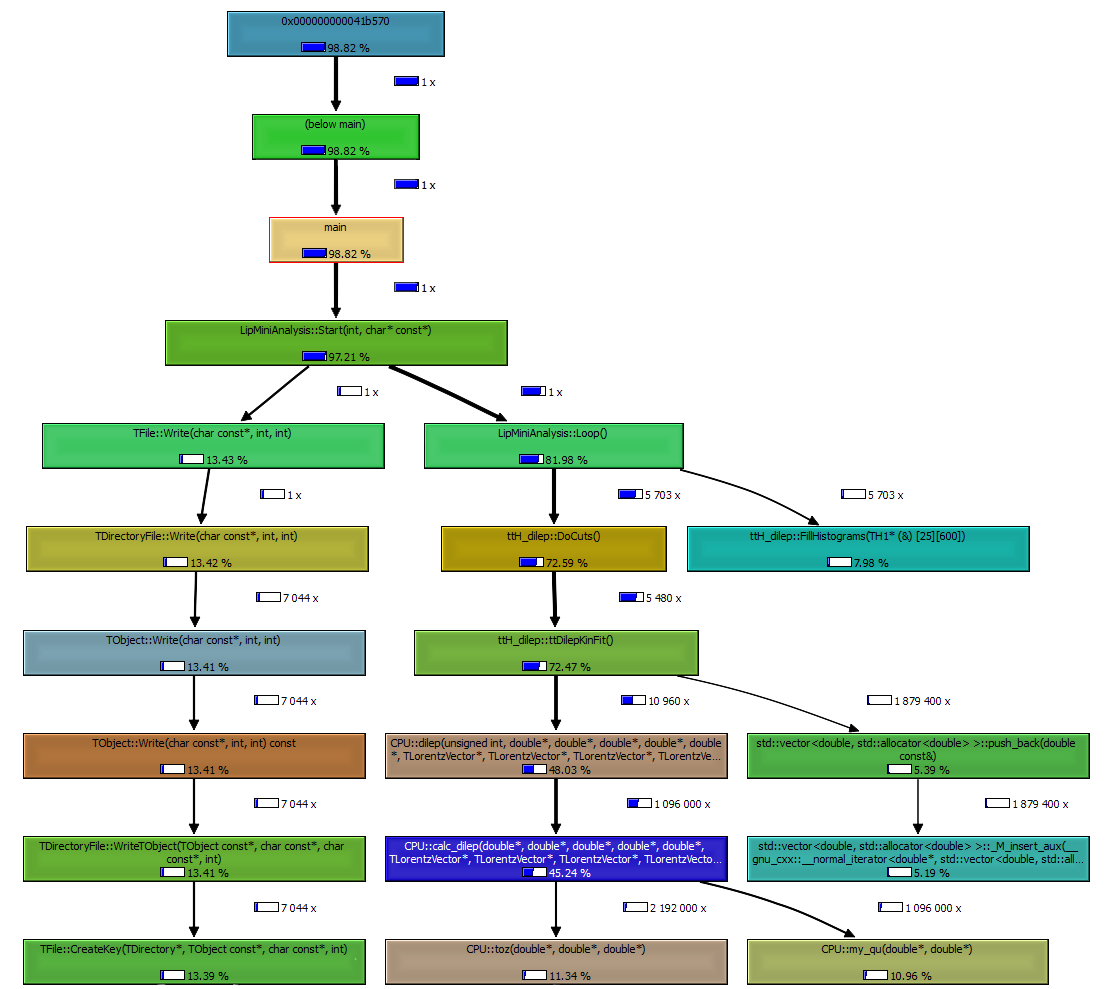
\includegraphics[scale=0.6]{../../common/img/callgraph_O3_100dilep.png}
		\caption{Callgraph generated using the Valgrind tool \cite{Callgrind} for the ttH\_dilep analysis with 100 dilep executions per event.}
		\label{fig:callgraph}
	\end{center}
\end{figure}

It is in this Tier-3 that the ttH\_dilep analysis application fits. It was developed by the LIP researchers to solve the problem explained in the section 2. The application has two main dependencies: the ROOT framework \cite{CERN:ROOT} and the LipMiniAnalysis library.

The ROOT framework is being developed by CERN and provides a set of functionalities needed to handle and analyze large amounts of data. They range from data storage, in the standard formats used by CERN, to histograming, curve fitting minimization and visualization methods. It aims to provide the programmer a set of tools that will ease the construction of their analysis code.

The LipMiniAnalysis is a library developed by LIP, containing a set of methods and functionalities useful for the analysis that they conduct with the ATLAS detector data. It is also prepared to read a more refined set of data resultant from the DPD data format that arrives at the Tier-3.

As illustrated by the callgraph of the analysis application in figure \ref{fig:callgraph}, the main flow of the application is controlled by the Loop method. This method will apply the DoCuts function to every event to process. The event passes a series of tests and evaluations (cuts). If an event reaches the cut 20, of a total of 21, the ttDilepKinFit function is called. It is in this function that the ttbar and Higgs reconstructions are performed. In the beginning of the ttDilepKinFit method, the available jets are combined two by two, as well as the leptons, as explained in section 2.

The dilep function, called after within the ttDilepKinFit method, analytically determines the neutrinos characteristics for each jets and leptons combination, reconstructing the ttbar system. It can produce two to four possible result particles. These results are used in the remaining of the ttDilepKinFit to determine the probability of the reconstruction, as well as reconstruct the Higgs boson. The final probability of the reconstruction is determined by combining the probability of the ttbar reconstruction with the calculated probability of the Higgs reconstruction.
As seen from the callgraph, most of the application execution time is spent in the Loop method, so there is the place where most efforts of optimization must be focused. The rest are auxiliary and I/O functions.

\newpage
